% !TeX root = Theo_IV.tex

\usepackage{tikz}
%\usepackage{pgfplots}
%\pgfplotsset{compat=1.18}

\usetikzlibrary{
    arrows.meta,
    bending,
    positioning,
    decorations.markings,
    intersections,
    calc,
    decorations.pathreplacing
}
%\tikzexternalize[prefix=figures/,shell escape=-enable-write18] % activate

\tikzset{
    % Colors
    object color/.style={blue!40!black!80!white},
    object style/.style={object color,thick},
    nice green/.style={green!50!black},
    nice orange/.style={red!60!yellow!70!black!90!white},
    nice dark blue/.style={blue!50!black},
    nice light blue/.style={blue!60!white!70!black},
    nice turquoise/.style={blue!50!green},
    polarisation color/.style={purple},
    charge color/.style={blue!50!white!70!black},
    red laser/.style={red!70!black},
    moving system color/.style={blue!60!black!70!white},
    %
    % Coordinate system
    coordsystem/.style={very thin, color=#1!50},
    xlabel/.style={anchor=north west},
    ylabel/.style={anchor=south east},
    %
    % Nodes and points
    invisible point/.style={circle,inner sep=0pt,outer sep=0pt,minimum size=0pt},
    point/.style={invisible point,fill=black,minimum size=4pt},
    %
    % Arrows
    arrow tip/.tip={Stealth},
    arr/.style={->,>={arrow tip}},
    rarr/.style={<-,>={arrow tip}},
    midarrow/.style={postaction=decorate,decoration={markings, mark=at position #1 with {\arrow[xshift=2.5pt]{arrow tip}}} },
    midarrow/.default=.5,
    rmidarrow/.style={postaction=decorate,decoration={markings, mark=at position #1 with {\arrowreversed{arrow tip}}} },
    rmidarrow/.default=.5,
    distance marker/.style={|<->|,>={arrow tip}},
}
\tikzstyle{every node}=[font=\footnotesize]


\newcommand{\tfigTitel}{
    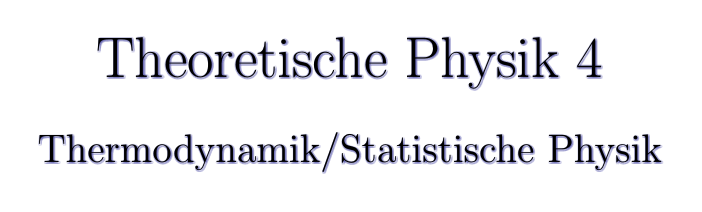
\begin{tikzpicture}
        \pgfmathsetmacro{\shadowangle}{132}
        \newlength{\shadowdistance}
        \pgfmathsetlength{\shadowdistance}{0.1ex}
        \pgfmathsetmacro{\shadowopacity}{1}
        \pgfmathsetmacro{\shadowspread}{0.003}
        \pgfmathsetmacro{\shadowsize}{5}
        \pgfmathtruncatemacro{\totshadow}{100}
        \path[nice dark blue,opacity={\shadowopacity/\totshadow},shift={({132-180}:\shadowdistance)},scale={1+\shadowsize}] 
        foreach \nshadow [evaluate=\nshadow as \angshadow using \nshadow/\totshadow*360] in {1,...,\totshadow}{
            node[align=center] at (\angshadow:\shadowspread) {\huge Theoretische Physik 4\\ \\ \\
            \Large Thermodynamik/Statistische Physik}
            };
        \node[align=center] at (0,0) {\huge Theoretische Physik 4\\ \\ \\ \Large Thermodynamik/Statistische Physik};
    \end{tikzpicture}
}
